\documentclass[./main.tex]{subfiles}

\begin{document}
    \subsubsection*{問5}
    \addcontentsline{toc}{subsubsection}{問5}
    \markboth{2024年 統計数理 問5}{2024年 統計数理 問5}


    \begin{enumerate}
        % Q1
        \item $X\sim U(-0.5, 0.5)$ の密度関数, 分布関数は
        $f(x) = 1_{ [ -0.5, 0.5) }$,
        $F(x) = \begin{cases}
            0 & (x < -0.5)\\
            x + \frac{1}{2} & (-0.5 \leq x < 0.5)\\
            1 & (0.5 \leq x)
        \end{cases}$


        \begin{alignat*}{2}
        &\therefore &\ &f_1 (x_1) = \frac{3!}{1!\,2!} f(x_1) \{ 1 - F(x_1) \}^2
            = 3 \left( 0.5 - x_1 \right)^2 \, 1_{[-0.5, 0.5)}\\
        &&&f_2 (x_2) = \frac{3!}{1! \, 1! \, 1!} F(x_2) f(x_2) \{ 1 - F(x_2) \}
            = 6 (0.25 - {x_2}^2) \, 1_{[-0.5, 0.5)}\\
        &&&f_3 (x_3) = \frac{3!}{2! \, 1!} \{ F(x_3) \}^2 f(x_3)
            = 3 (x_3 + 0.5)^2 \, 1_{[-0.5, 0.5)}
        \end{alignat*}
        また $\displaystyle E[X_{(1)}] = \int_{-0.5}^{0.5} x_1 \cdot 3 (0.5 - x_1)^2 \, dx_1
            = -3 \cdot 2 \int_0^{0.5} {x_1}^2 \, d x_1
            = - \frac{1}{4}$, 
        $E [X_{(2)}]$ は奇関数の積分で $0$, $E [X_{(3)}]$ は $E [X_{(1)}]$ と逆向きの積分で $\dfrac{1}{4}$.

        % $X_{(1)}, X_{(2)}, X_{(3)}$ の分布関数をそれぞれ $F_1(x_1), F_2 (X_2), F_3 (x_3)$ とすると


        % Q2
        \item $f(x_1, x_2, x_3) = 3! \, f(x_1) f(x_2) f(x_3) \, 1_{\{ x_1 \leq x_2 \leq x_3 \}}
            = 6 \cdot 1_{\{ -0.5 \leq x_1 \leq x_2 \leq x_3 < 0.5 \}}$
            % = 6 \cdot 1_{x_1 : x_1 \in [-0.5, 0.5)}1_{x_2 : x_2 \in [-0.5, 0.5)} 1_{x_3 : x_3 \in [-0.5, 0.5)}
            %    1_{\{ x_1 \leq x_2 \leq x_3 \}}$

        % Q3
        \item $\hat{\theta}_c
            = c (X_{(1)} + \theta) + (1 - 2c) (X_{(2)} + \theta) + c(X_{(3)} + \theta)
            = c X_{(1)} + (1 - 2c) X_{(2)} + c X_{(3)} + \theta$ より, \\
            $E [\hat{\theta}_c] = c E[X_{(1)}] + (1 - 2c) E[X_{(2)}] + c E[X_{(3)} ] + \theta
                = \theta$.
            よって不偏。
        
        % Q4
        \item $Y_{(1)}, Y_{(2)}, Y_{(3)}$ の同時確率密度関数 $f_{Y_{(1)}, Y_{(2)}, Y_{(3)}} (y_1, y_2, y_3)$ は
        \begin{equation*}
            f_{Y_{(1)}, Y_{(2)}, Y_{(3)}} (y_1, y_2, y_3)
                = 6 \cdot 1_{ \{ - 0.5 + \theta \leq y_1 \leq y_2 \leq y_3 < 0.5 + \theta \}}
                = 6 \cdot 1_{ \{y_3 - 0.5 < \theta \leq y_1 + 0.5 \} } \cdot 1_{ \{ y_1 \leq y_2 \leq y_3 \}}
        \end{equation*}
        よって Fisher-Neyman の因子分解定理より、$\{ Y_{(1)}, Y_{(3)} \}$ は $\theta$ に関する十分統計量。

        % Q5
        \item $Y_{(1)}, Y_{(3)}$ の周辺確率密度関数 $f_{Y_{(1)}, Y_{(3)}} (y_1, y_3)$ は
        \begin{equation*}
            f_{Y_{(1)}, Y_{(3)}} (y_1, y_3)
                = \int f_{Y_{(1)}, Y_{(2)}, Y_{(3)}} (y_1, y_2, y_3) \, dy_2
                % = 6 \cdot 1_{ \{y_3 - 0.5 < \theta \leq y_1 + 0.5 \} } \int_{y_1}^{y_3} \, dy_2
                = 6(y_3 - y_1) \cdot 1_{ \{y_3 - 0.5 < \theta \leq y_1 + 0.5 \} } 
        \end{equation*}
        よって条件付き確率密度関数は
        \begin{equation*}
            f_{Y_{(2)} \mid Y_{(1)}, Y_{(3)}} ( y_2 \mid y_1, y_3)
                = \frac{f_{Y_{(1)}, Y_{(2)}, Y_{(3)}} (y_1, y_2, y_3)}{f_{Y_{(1)}, Y_{(3)}} (y_1, y_3)}
                = \frac{1}{y_3 - y_1} \cdot 1_{ \{ y_1 \leq y_2 \leq y_3 \}}
        \end{equation*}
        したがって
        \begin{equation*}
            E[ Y_{(2)} \mid Y_{(1)} = y_{1}, Y_{(3)} = y_{3}]
                = \int y_2 \, f_{Y_{(2)} \mid Y_{(1)}, Y_{(3)}} ( y_2 \mid y_1, y_3) \, dy_2
                = \frac{y_1 + y_3}{2}
        \end{equation*}
        すなわち、$\displaystyle E[ Y_{(2)} \mid Y_{(1)}, Y_{(3)}] = \frac{Y_{(1)} + Y_{(3)}}{2}$.
        ところで、$\hat{\theta}_c$ は不偏であったから、Rao-Blackwell の定理により
        \begin{align*}
            \hat{\theta}^*
                &= E [\hat{\theta}_c \mid Y_{(1)}, Y_{(3)}]\\
                &= c (Y_{(1)} + Y_{(3)}) + (1 - 2c) \frac{Y_{(1)} + Y_{(3)}}{2}\\
                &= \frac{Y_{(1)} + Y_{(3)}}{2}
        \end{align*}
        で定義される新たな推定量 $\hat{\theta}^*$ もまた不偏で、その分散は任意の $\hat{\theta}_c$ の分散以下になる。
        よって、$\hat{\theta}_c = \hat{\theta}^*$ をみたす $c$ が存在すればその $c$ において $V[\hat{\theta}_c]$ が最小になるが、
        実際そのような $c$ は存在して、$c = \frac{1}{2}$ である。
    \end{enumerate}


    % ~~~~~~~~~~~~~~~~~~~~~~~~~~~~~~~~~~~~~~~~~~~~~~~~~~~~~~~~~~~~~~~~~~~~~~~~~~~~~~~~~~
    \subsubsection*{コメント}
    順序統計量\index{順序統計量}はとっても難しいけど、メタな話、一様分布\index{一様分布}くらいしか出ないので一通りやり方をさらっておこう。
    場合分けはいちいち書いていると脳が破壊されるので、適宜指示関数\index{指示関数}を使いながら機械的に処理できるようにしておくとよい
    (指示関数に拘って逆に混乱しないように)。
    最後は Rao-Blackwell の定理で不偏推定量の分散を小さくする話ができたら Good.

    しかし 2024年の統計数理、内容が被るねぃ。
    全体的に尤度ばっかりだし、問2 でも最大統計量の話が出てた。
    因子分解定理も問3 に出てたし。
    人によってはチャンスの年だったのかもしれませんね。
    \begin{enumerate}
        % Q1
        \item 難しいけどワンパターンな順序統計量。
        最大統計量 $X_{(3)}$ や最小統計量 $X_{(1)}$ の密度関数に関しては累積分布を考えると分かりやすいですが
        (同じく 2024 年 統計数理 問2 [3] の答案ではその方針で書きました)、
        中央値 $X_{(2)}$ はそう簡単には行かないので、
        答案では一律密度関数を直接求める方針で書いています。
        プロセスは \cite{kubokawa:2017} に分かりやすく書かれてあるので一読をおすすめします。

        % Q2
        \item $X_{(1)}, X_{(2)}, X_{(3)}$ は独立ではないので同時確率密度関数はシンプルなかけ算にはなりません。
        3 変数の並び順の任意性 $(3!)$ と、$x_1, x_2, x_3$ の大きさ順の制限 $1_{\{ x_1 \leq x_2 \leq x_3 \}}$ が掛かります。

        % Q3
        \item この時点では謎めいた問いですが、$\hat{\theta}_c$ の不偏性があとあと活きていくことになります。
        
        % Q4
        \item 十分統計量\index{じゅうぶんとうけいりょう@十分統計量}といえば因子分解定理\index{いんしぶんかいていり@因子分解定理}です。
        今回は同時確率密度関数 $f_{Y_{(1)}, Y_{(2)}, Y_{(3)}} (y_1, y_2, y_3)$ において、 $\theta$ が
        $\{ y_1, y_3 \}$ を通してのみ依存することを示したいですが、
        指示関数の不等号が
        \begin{equation*}
            - 0.5 + \theta \leq y_1 \leq y_2 \leq y_3 < 0.5 + \theta 
        \end{equation*}
        のように両端に $\theta$ が来る形になるおかげで $y_2$ の条件を分離でき、
        \begin{equation*}
            y_3 - 0.5 < \theta \leq y_1 + 0.5 \quad \text{and} \quad
            y_1 \leq y_2 \leq y_3
        \end{equation*}
        のように言い換えることができるということですね。
        指示関数を使えるとこういった操作の時の記述量や思考リソースを下げられるので便利です。

        % Q5
        \item 不偏推定量, 十分統計量, 条件付き期待値\index{じょうけんつききたいち@条件付き期待値}... と聞いて、
        Rao-Blackwell の定理\index{らおぶらっくうぇるのていり@Rao-Blackwell の定理}を想像できたでしょうか？という問題です。
        できませんでしたか？安心してください！ここで勉強すればよいのです。

        \begin{theorem}[Rao-Blackwell の定理]
            $\theta$ の不偏推定量 $\hat{\theta}$ ( すなわち $E[\hat{\theta}] = \theta$ ) と
            十分統計量 $T$ が与えられる。
            この時、$\hat{\theta}$ を $T$ で条件付けた
            \begin{equation*}
                \hat{\theta}^* = E[\hat{\theta} \mid T]
            \end{equation*}
            という新たな推定量 $\hat{\theta}^*$ もまた $\theta$ の不偏推定量であり、
            かつその分散は $\hat{\theta}$ の分散を超えない。
            \begin{equation*}
                E[\hat{\theta}^*] = \theta, \qquad
                V[\hat{\theta}^*] \leq V [\hat{\theta}]
            \end{equation*}
        \end{theorem}

        \ \\つまり、不偏推定量と十分統計量を使って、もとの推定量よりも悪くはない不偏推定量を新たに作ることができるというのが、
        この定理の主張することです。
        このようにして分散を小さくしていくことを Rao-Blackwellization と言ったりします。

        なお、より一般に $\hat{\theta}$ が不偏でない場合の Rao-Blackwell の定理も成立します。
        その場合は平均二乗誤差が小さくなるという表現になります (証明を見れば分かりますが結局分散も小さくなります)。
        % 証明はそちらの方でまとめて行うことにします。

        \begin{theorem}[Rao-Blackwell の定理]
            $\theta$ の推定量 $\hat{\theta}$ と
            十分統計量 $T$ が与えられる。
            この時、$\hat{\theta}$ を $T$ で条件付けた
            \begin{equation*}
                \hat{\theta}^* = E[\hat{\theta} \mid T]
            \end{equation*}
            という新たな推定量 $\hat{\theta}^*$ は $\hat{\theta}$ と同じ期待値を持ち、
            かつその平均二乗誤差は $\hat{\theta}$ の平均二乗誤差を超えない。
            \begin{equation*}
                E[\hat{\theta}^*] = E[\hat{\theta}], \qquad
                E[( \hat{\theta}^* -\theta)^2 ] \leq E [(\hat{\theta} - \theta)^2]
            \end{equation*}
        \end{theorem}
        \ 
        \begin{proof}
            \small
            期待値については繰り返し期待値の法則 (tower law) により 
            $E[\hat{\theta}^*] = E[  E[\hat{\theta} \mid T]]
                = E [\hat{\theta}]$.
            平均二乗誤差については、bias-variance 分解により
            \begin{align*}
                E[( \hat{\theta}^* -\theta)^2 ] 
                    &=  E [ ( E[\hat{\theta}^*] - \theta)^2 ] + V [ \hat{\theta}^* ]\\
                E [(\hat{\theta} - \theta)^2]
                    &=  E [ ( E[\hat{\theta}] - \theta)^2 ] + V [ \hat{\theta} ]
            \end{align*}
            となり、$ E[\hat{\theta}^*] = E[\hat{\theta}] $ より
            両者のバイアス項は等しいため、分散の大小を比較すれば良いことになる。
            ここで全分散の公式\index{ぜんぶんさんのこうしき@全分散の公式} 
            $V[X] = E[ V[X \mid Y]] + V [ E [X \mid Y]]$ により
            \begin{equation*}
                V[\hat{\theta}] = E [ V [\hat{\theta} \mid T]] + V[ E[\hat{\theta} \mid T]]
            \end{equation*}
            であり、右辺第 2 項は $V[\hat{\theta}^*]$, 右辺第 1 項は 0 以上となるため、
            $V[\hat{\theta}] \geq V[\hat{\theta}^*]$.
        \end{proof}

        なお、(下に) 凸関数 $\phi$ に関する Jensen の不等式\index{いぇんせんのふとうしき@Jensen の不等式}
        :  $\phi(E[X]) \leq E[\phi(X)] $ (図 \ref{fig:2024-suri-5-jensen}) を使って示すこともできる
        \footnote{以下の証明でつかっているのは $\phi(x) = x^2$ の場合であるため、実質コーシー・シュワルツの不等式と変わらない。
        何なら分散が 0 以上であるという条件を使っているだけであるとも言える。
        なのに何故に Jensen を持ち出すかというと、実は平均二乗誤差よりもさらに広い関数に対して
        同様の不等号が成り立ちそうな雰囲気がありそうなことをそれとなく仄めかしたかったからである。}。

        % Jensen の不等式
        \begin{figure}[tb]
            \centering
            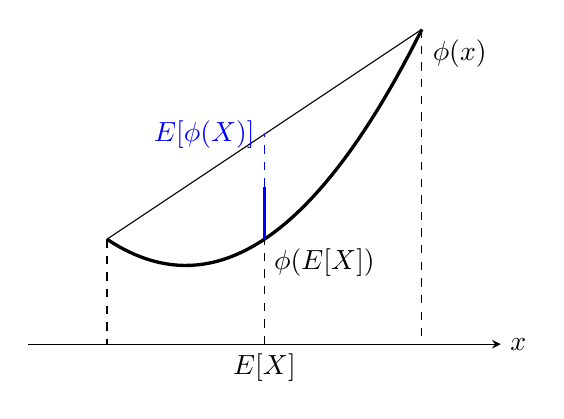
\begin{tikzpicture}
                \draw[-stealth] (-2, 0)--(4, 0) node[right] {$x$};
                \draw[very thick, domain=-1:3, samples=50] plot (\x, \x*\x / 3 + 1) node[below right] {$\phi(x)$};

                \draw (-1, 4/3) -- (3, 4);
                \draw [blue, dashed] (1, 6/3) -- (1, 8/3) node[left] {$E[\phi (X) ]$};
                \draw [thick, blue] (1, 4/3) -- (1, 6/3);

                \draw [dashed] (1, 0) node[below] {$E[X]$} -- (1, 4/3) node[below right] {$\phi( E[X])$};
                \draw [dashed] (-1, 4/3) -- (-1, 0);
                \draw [dashed] (3, 4) -- (3, 0);
            \end{tikzpicture}
            \caption{Jensen の不等式 $\phi(E[X]) \leq E[\phi(X)]$ の図形的解釈。
            図は必ずしも正確とは限りません}
            \label{fig:2024-suri-5-jensen}
        \end{figure}
        \begin{proof}
            \small
            \begin{align*}
                &E[ (\hat{\theta}^* - \theta)^2]\\
                &= E \left[ ( E[\hat{\theta} \mid T] - \theta )^2 \right]
                = E \left[ ( E[\hat{\theta} - \theta \mid T])^2 \right]
                \leq E \left[ E[ (\hat{\theta} - \theta)^2 \mid T] \right]
                = E [(\hat{\theta} - \theta)^2].
            \end{align*}
        \end{proof}

    \end{enumerate}

\end{document}